\documentclass[
12pt, % Main document font size
a4paper, % Paper type, use 'letterpaper' for US Letter paper
oneside, % One page layout (no page indentation)
%twoside, % Two page layout (page indentation for binding and different headers)
%hidelinks, % Hide links like hyperref
%headinclude,footinclude, % Extra spacing for the header and footer
%BCOR5mm, % Binding correction
]{article}



%\setlength{\parindent}{0pt} %Modifica la dimensione dell'indentazione dei paragrafi



\hyphenation{Fortran hy-phen-ation se-mi-auto-no-} 


%%%%% Packages
\usepackage [italian]{babel}
%\usepackage [english]{babel}
\usepackage [autostyle, english = american]{csquotes}
\MakeOuterQuote{"}

\usepackage[section]{placeins} %Also one can consider the placeins package and the \FloatBarrier command that prevents figures from floating any further. If figures are supposed to remain in the section, one can load

\usepackage{graphicx}
\usepackage{subfig}
\usepackage{xcolor} %Colori Aggiuntiv
\usepackage[colorlinks = true,
	linkcolor = teal,
	urlcolor  = blue,
	citecolor = blue,
	anchorcolor = blue]{hyperref} %Hyperref
	
\usepackage{url}

%\usepackage{lipsum} %Crea dummy text

\usepackage{amsmath,amssymb,amscd,amsfonts,amsthm,amsrefs} %Roba matematica
\usepackage{mathtools}

\usepackage{physics}

\usepackage{siunitx} %database unita` di misura, \si{ \kg \per \second},  \SI{20}{ \kg \per \second}

\usepackage{gensymb} %simboli extra, come \degree

\usepackage{tikz}
	\usetikzlibrary{shapes,arrows}
	\tikzstyle{block} = [draw, fill=white, rectangle, 
	minimum height=3em, minimum width=6em]
	\tikzstyle{sum} = [draw, fill=white, circle, node distance=1cm]
	\tikzstyle{input} = [coordinate]
	\tikzstyle{output} = [coordinate]
	\tikzstyle{pinstyle} = [pin edge={to-,thin,black}]
	\usepackage{tikzscale}

\usepackage{pgfplots}
	\pgfplotsset{width=7cm,compat=1.14}
	%\pgfplotsset{compat=newest} % Allows to place the legend below plot
	\pgfplotsset{every minor tick/.append style={thin}}  % applies only to minor ticks,
	\usepgfplotslibrary{units} % Allows to enter the units nicely
	%\usepgfplotslibrary{external} 
	%\tikzexternalize
	%\tikzset{external/force remake}
	\pgfkeys{/pgf/number format/.cd,1000 sep={\,}}

\sisetup{
	round-mode          = places,
	round-precision     = 2,
}



\usepackage{afterpage}

\newcommand\blankpage{%
	\null
	\thispagestyle{empty}%
	%\addtocounter{page}{-1}%
	\newpage}
%per creare pagine vuote

\usepackage{vmargin}
\setmarginsrb  {25mm}  % left margin
	{ 5mm}  % top margin
	{25mm}  % right margin
	{15mm}  % bottom margin
	{10mm}  % head height
	{15mm}  % head sep
	{10mm}  % foot height
	{15mm}  % foot sep

\setpapersize{A4}


%%%%%%%%%%%%%%%%%%%%%%%%%%%%%%%%%%%%%%%%%%%%%%%%%%%%%%%%%%
%%%%% Comandi homebrewed

\newcommand{\at}[2][]{#1|_{#2}} %Comando per le derivate calcolate nel punto. Esempio: \dv{\text{Im}T(j \omega)}{t} \at[\Big]{\omega = \omega_1}

%% Comando per valori assoluti che scalano
%\DeclarePairedDelimiter\abs{\lvert}{\rvert}%
%\DeclarePairedDelimiter\norm{\lVert}{\rVert}%
% Swap the definition of \abs* and \norm*, so that \abs
% and \norm resizes the size of the brackets, and the 
% starred version does not.
\makeatletter
\let\oldabs\abs
\def\abs{\@ifstar{\oldabs}{\oldabs*}}
%
\let\oldnorm\norm
\def\norm{\@ifstar{\oldnorm}{\oldnorm*}}
\makeatother

\DeclarePairedDelimiter\ceil{\lceil}{\rceil}
\DeclarePairedDelimiter\floor{\lfloor}{\rfloor}

%% Prova theorem
\newtheorem{theorem}{Theorem}[section]
\newtheorem{lemma}[theorem]{Lemma}
\newtheorem{proposition}[theorem]{Proposition}
\newtheorem{corollary}[theorem]{Corollary}

\newenvironment{Proof}[1][Proof]{\begin{trivlist}
		\item[\hskip \labelsep {\bfseries #1}]}{\end{trivlist}}
\newenvironment{definition}[1][Definition]{\begin{trivlist}
		\item[\hskip \labelsep {\bfseries #1}]}{\end{trivlist}}
\newenvironment{example}[1][Example]{\begin{trivlist}
		\item[\hskip \labelsep {\bfseries #1}]}{\end{trivlist}}
\newenvironment{remark}[1][Remark]{\begin{trivlist}
		\item[\hskip \labelsep {\bfseries #1}]}{\end{trivlist}}

%\newcommand{\qed}{\nobreak \ifvmode \relax \else
%	\ifdim\lastskip<1.5em \hskip-\lastskip
%	\hskip1.5em plus0em minus0.5em \fi \nobreak
%	\vrule height0.75em width0.5em depth0.25em\fi}




\graphicspath{{./figs/}}
\pgfplotsset{
	table/search path={./figs},
}

\title{\normalfont{Simulazione e Controllo del Pendolo Inverso di Furuta}}
\author{Francesco Petracci e Simone Silenzi} 


\begin{document}


\begin{titlepage}
	\centering
	\vspace*{2 cm}
	\textsc{\Large Universit\`a di Pisa }\\[0.5 cm]							% University Name
	%\textsc{\Large Scuola di Ingegneria}\\[0.5 cm]		
	\textsc{\large Corso di Laurea magistrale \\ 
		\vspace*{3mm} in Ingegneria Robotica e dell'Automazione}\\[1 cm]		% Course Code
	\rule{\linewidth}{0.2 mm} \\
	{ \Large{\textbf{Simulazione e Controllo \\ del Pendolo Inverso di Furuta}}}\\
	
	\rule{\linewidth}{0.2 mm} \\[2.5 cm]
%	\vspace*{1.5 cm}
	
	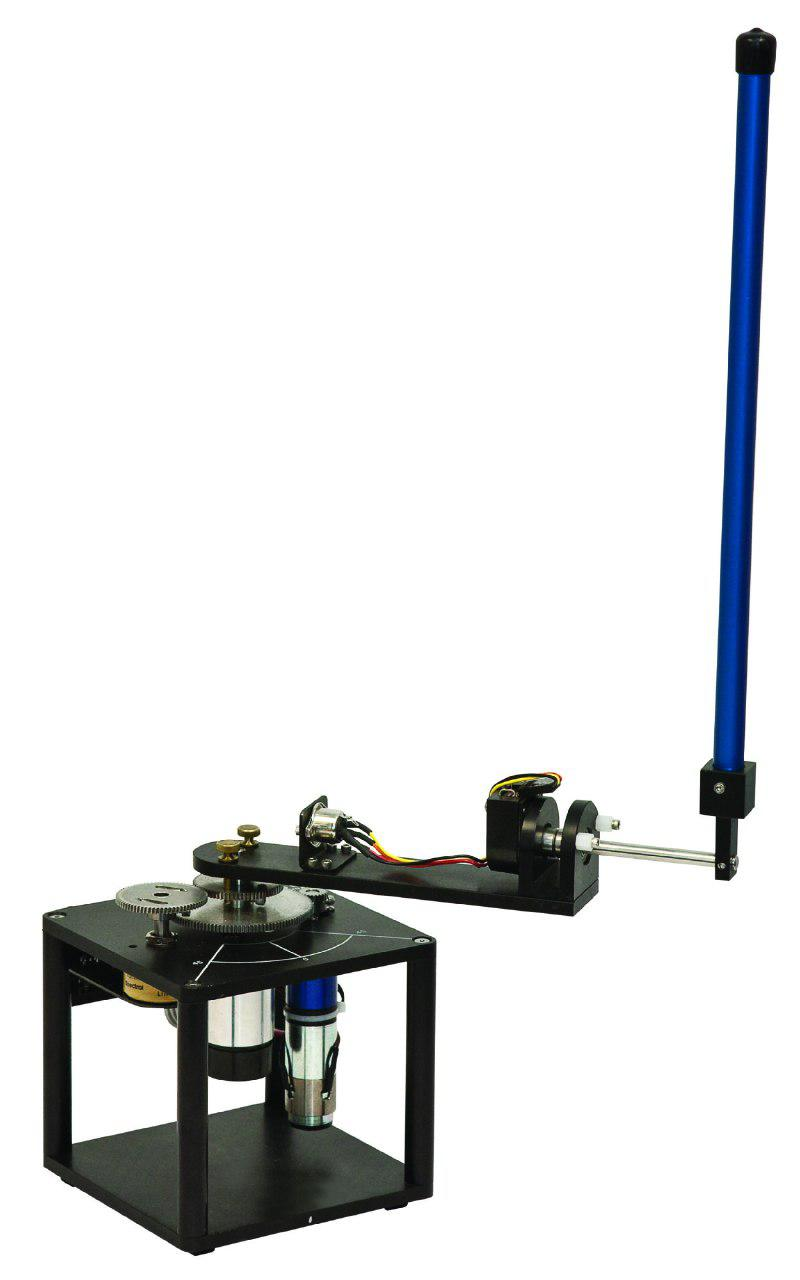
\includegraphics[height=.35\textheight]{quanser_furuta1.jpg}
	
	\vspace*{2 cm}
	\begin{minipage}{0.48\textwidth}
		\begin{flushleft}
			\textit{Autori:}\\
			Francesco Petracci\\
			Simone Silenzi
		\end{flushleft}
	\end{minipage}~
	\begin{minipage}{0.48\textwidth}
		\begin{flushright}
			\textit{Matricola e-mail:}\\		
			491648, \href{mailto:petracci.francesco@gmail.com}{petracci.francesco@gmail.com} \\
			460123, \href{mailto:s.silenzi1@gmail.com}{s.silenzi1@gmail.com}
		\end{flushright}
	\end{minipage}\\[2 cm]
	
%	\textit{Autori, matricola ed email:} \\
%	Francesco Petracci, 491648, \href{mailto:petracci.francesco@gmail.com}{petracci.francesco@gmail.com} \\
%	Simone Silenzi, 460123, \href{mailto:s.silenzi1@gmail.com}{s.silenzi1@gmail.com} \\
	
	
\end{titlepage}
\newpage

\section{Indicazioni Report}
Project reportA  report  must  be  produced  (8-10  pages)  to  explain  the  project  details.  In  particular,  the  title  page  must  contain  the  name  of  the  course  under  which  the  project  has  been  done,  the  project  title,  an  optional  picture related  to  the  project,  the  delivery  date,  and the  author(s)  name(s)  with  contact  information (student ID number and Email). The  report  must  include  a  general  description  of  the  project,  the  physical  model  used,  the  design  choices, the user interface, the shared data structures, the tasks involved, a task-resource diagram, a discussion  on  the  task  parameters  (how they  were  defined),  and  a  set  of  experimental  results  that show  the  behavior  of  the  system  as  a  function  of  specific  variables.  Figures  and  screen  shots  are  welcome. The project code must not be included in the report, but in a separate folder.

TO DO LIST:
\begin{itemize}
	\item RIFARE SCHEMA PENDOLO,primo link da rifare il cilindro finale
	\item AGGIORNARE la parte sulla grafica in modo da rispiecchiare drawings.m
	\item Conclusioni
\end{itemize}
 
\section{Introduzione}
Questo progetto consiste nella simulazione dell'interazione real-time tra il pendolo inverso di Furuta, una scheda STM32F4 Discovery e un'interfaccia utente su pc. 

L'applicazione finale \`e stata sviluppata in C sfruttando principalmente le librerie Allegro e Pthread. Per quanto riguarda la simulazione del pendolo e della scheda \`e stato fatto uso del software \textsc{Matlab--Simulink} per sviluppare un modello fisico, il relativo controllo e per quindi creare in modo automatico alcune funzioni.


\section{cose Simone}
\begin{math}\\
T=\dfrac{1}{2} \left(2  L_{arm} l_p m_p \dot{\alpha } \dot{\theta } \cos (\theta ) + \left(J_0 + J_p\sin ^2(\theta )\right) \dot{\alpha }^2+ J_p \dot{\theta }^2\right)\\
U=g l_p m_p (\cos(\theta) - 1)\\
M(q)\ddot{q}+C(q,\dot{q})\dot{q}+N(q,\dot{q})=\tau\\
q=\left( \begin{array}{cc}\alpha & \theta\\\end{array}\right)^{T}\\
M(q)=\left(\begin{array}{cc}\dfrac{\partial^{2} T}{\partial \dot{\alpha }^{2} } & \dfrac{\partial^{2} T}{\partial \dot{\alpha } \partial \dot{\theta } }\\
\dfrac{\partial^{2} T}{\partial \dot{\alpha } \partial \dot{\theta } } & \dfrac{\partial^{2} T}{\partial \dot{\theta }^{2} }\\
\end{array}\right)=\left(\begin{array}{cc}
J_0+J_p \sin ^2(\theta ) & L_{arm} l_p m_p \cos (\theta ) \\
L_{arm} l_p m_p \cos (\theta ) & J_p \\
\end{array}\right)\\
C(q,\dot{q})= \dfrac{1}{2}\left(
\begin{array}{cc}
\dfrac{\partial M_{11}}{\partial \alpha}\dot{\alpha } + \dfrac{\partial M_{11}}{\partial \theta}\dot{\theta } &
\dfrac{\partial M_{11}}{\partial \theta}\dot{\alpha } + (2 \dfrac{\partial M_{12}}{\partial \theta} - \dfrac{\partial M_{22}}{\partial \alpha})\dot{\theta } \\
(2 \dfrac{\partial M_{21}}{\partial \alpha} - \dfrac{\partial M_{11}}{\partial \theta}) \dot{\alpha } + \dfrac{\partial M_{22}}{\partial \alpha} \dot{\theta } &
\dfrac{\partial M_{22}}{\partial \alpha} \dot{\alpha } + \dfrac{\partial M_{22}}{\partial \theta} \dot{\theta }\\
\end{array}\right) = \left(	\begin{array}{cc}\dfrac{1}{2} J_p \dot{\theta } \sin (2 \theta )& \dfrac{1}{2} J_p \dot{\alpha } \sin (2 \theta )-L_{arm} l_p m_p\dot{\theta } \sin (\theta ) \\
-\dfrac{1}{2} J_p \dot{\alpha } \sin (2 \theta ) & 0 \\
\end{array}
\right)\\
N(q,\dot{q})=\left(\begin{array}{c}b_{ma}\dot{\alpha } + \dfrac{\partial U}{\partial \alpha }\\
b_p \dot{\theta } + \dfrac{\partial U}{\partial \theta }\\
\end{array}\right)=\left(\begin{array}{c}
b_{ma} \dot{\alpha }\\
b_p \dot{\theta } -g l_p m_p \sin (\theta )\\
\end{array}\right)\\
\ddot{q}={M(q)}^{-1}(\tau-C(q,\dot{q})\dot{q}-N(q,\dot{q}))\\
\left(\begin{array}{c}\ddot{\alpha}\\
\ddot{\theta}\\
\end{array}\right) ={\left(\begin{array}{cc}
	J_0+J_p \sin ^2(\theta ) & L_{arm} l_p m_p \cos (\theta ) \\
	L_{arm} l_p m_p \cos (\theta ) & J_p \\
	\end{array}\right)}^{-1}\left(\left(\begin{array}{c}\tau_1\\\tau_2\\\end{array}\right)-\left(
\begin{array}{cc}\dfrac{1}{2} J_p \dot{\theta } \sin (2 \theta )&\dfrac{1}{2} J_p \dot{\alpha } \sin (2 \theta )-L_{arm} l_p m_p\dot{\theta } \sin (\theta ) \\
-\dfrac{1}{2} J_p \dot{\alpha } \sin (2 \theta ) & 0 \\
\end{array}
\right)\left( \begin{array}{c}\dot{\alpha}\\
\dot{\theta}\\
\end{array}\right)-\left(\begin{array}{c}
b_{ma} \dot{\alpha }\\
b_p \dot{\theta } -g l_p m_p \sin (\theta )\\
\end{array}\right)\right)
%	=\\=\left(\begin{array}{c}
%		\dfrac{2 \dot{\theta } L_{arm} b_p \cos (\theta ) l_p m_p-2 g L_{arm} \sin
%			(\theta ) \cos (\theta ) l_p^2 m_p^2+\dot{\alpha }^2 L_{arm} \sin (2 \theta )
%			(-\cos (\theta )) J_p l_p m_p+2 \dot{\theta }^2 L_{arm} \sin (\theta ) J_p l_p
%			m_p-2 \tau _2 L_{arm} \cos (\theta ) l_p m_p-2 \dot{\alpha } b_{ma} J_p-2
%			\dot{\alpha } \dot{\theta } \sin (2 \theta ) J_p^2+2 \tau _1 J_p}{2
%			\left(-L_{arm}^2 \cos ^2(\theta ) l_p^2 m_p^2+\sin ^2(\theta ) J_p^2+J_0
%			J_p\right)} \\
%		\dfrac{2 \dot{\alpha } L_{arm} b_{ma} \cos (\theta ) l_p m_p+2 \dot{\alpha }
%			\dot{\theta } L_{arm} \sin (2 \theta ) \cos (\theta ) J_p l_p m_p-2 \tau _1
%			L_{arm} \cos (\theta ) l_p m_p-2 \dot{\theta }^2 L_{arm}^2 \sin (\theta )
%			\cos (\theta ) l_p^2 m_p^2-2 \dot{\theta } J_0 b_p-2 \dot{\theta } b_p \sin ^2(\theta )
%			J_p+2 g \sin ^3(\theta ) J_p l_p m_p+2 g J_0 \sin (\theta ) l_p m_p+\dot{\alpha }^2 \sin
%			(2 \theta ) \sin ^2(\theta ) J_p^2+\dot{\alpha }^2 J_0 \sin (2 \theta ) J_p+2 \tau _2
%			\sin ^2(\theta ) J_p+2 J_0 \tau _2}{2 \left(-L_{arm}^2 \cos ^2(\theta ) l_p^2
%			m_p^2+\sin ^2(\theta ) J_p^2+J_0 J_p\right)} \\
%	\end{array}\right)
\end{math}

\section{Modello}
\label{sez:modello}
Da scrivere

\section{Controllo}
\label{sez:controllo}
Da scrivere

\section{Interfaccia}
\label{sez:interfaccia}

\begin{figure}[]
	\centering
	%\def\svgwidth{0.7\linewidth}
	%\input{schema_2.pdf_tex}
	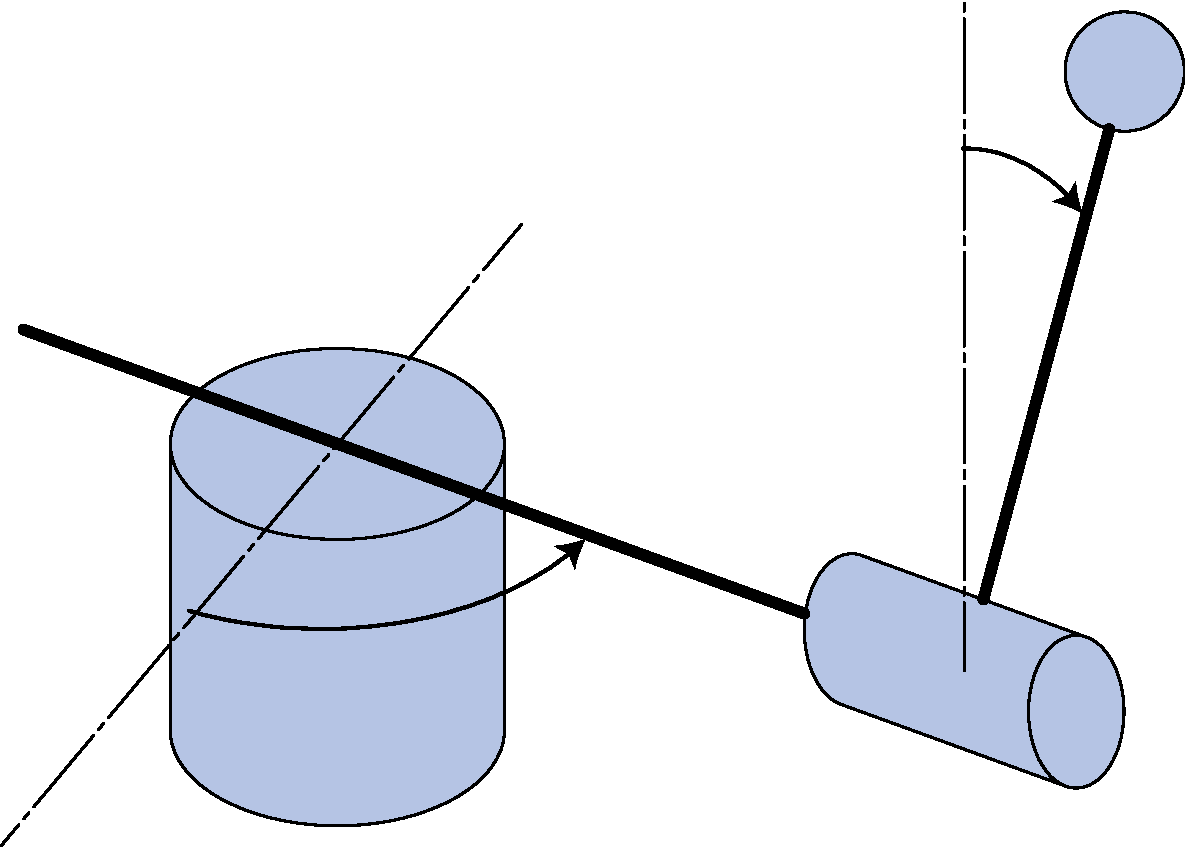
\includegraphics[width=.7\linewidth]{schema_2.pdf}
	\caption{Schema del Pendolo \textbf{DA SISTEMAREE}}
	\label{fig:pendolo_schema}
\end{figure}

\begin{figure}[]
	\centering
	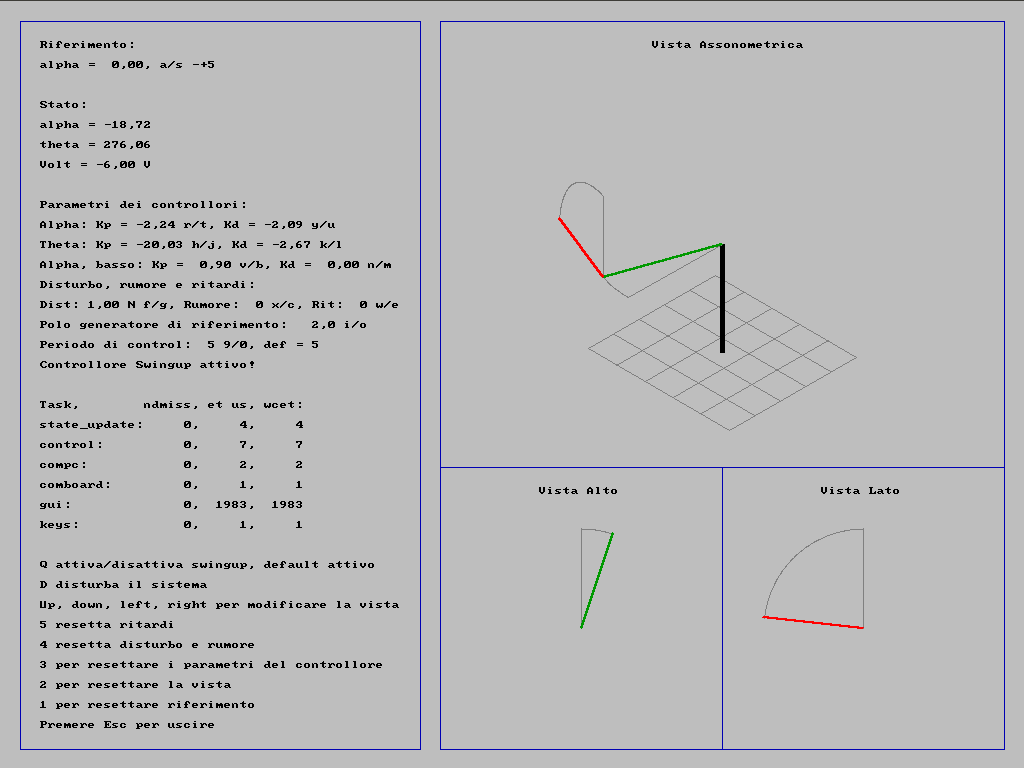
\includegraphics[height=.4\textheight]{interfaccia_in_esecuzione.png}
	\caption{Interfaccia durante l'esecuzione}
	\label{fig:interfaccia_in_esecuzione}
\end{figure}
L'interfaccia \`e divisa in due zone principali: quella di comunicazione con l'utente e le tre viste del pendolo.
Per quanto riguarda la zona di comunicazione questa \`e popolata dalle variabili di interesse e di come modificarle. Si \`e quindi riportato a schermo:
\begin{itemize}
	\item il riferimento su $\alpha$
	
	\item  il vettore di stato $\left[ \alpha \ \theta \ volt\right]^T$
	
	\item i parametri di controllo
	
	\item disturbo, rumore e ritardi
	
	\item polo della funzione di trasferimento che genera il riferimento su $\alpha$
	
	\item periodo del task di controllo
	
	\item per ciascun task il numero di deadline miss, il tempo di esecuzione in $\si{\micro \second}$ e il worst-case execution time in $\si{\micro \second}$
	
	\item varie istruzioni su come resettare e come uscire dal programma
	
\end{itemize}
Per quanto riguarda le viste, queste sono tre. La vista dall'alto evidenzia il primo link e quindi \`e possibile vedere $\alpha$ mentre in quella da lato $\theta$.

Per costruire la vista assonometrica \`e stato utile strutturare il problema in coordinate omogenee e introdurre dei sistemi di riferimento ausiliari. Tenendo d'occhio la figura~\ref{fig:pendolo_schema} e intendendo con $R_i(\varphi)$ la generica rotazione intorno all'asse $i$ di un angolo $\varphi$ e con $T_{ij}$ la trasformazione in coordinate omogenee dal sistema di riferimento $i$ a quello $j$ tale che per un generico vettore $p$ valga: $^ip = T_{ij}\ ^j p$; si pu\`o elaborare i cambi di coordinate necessari. 
\begin{equation}
	^0\! T_{01}(\alpha) = \left[ \begin{array}{ccc|c}
	& & & l_1 \\
	& R_z(\alpha) & & 0 \\
	& & & 0 \\
	\hline
	0 & 0 & 0 & 1
	\end{array} \right]
	\quad 
	^1 T_{12}(\vartheta) =
	\left[  \begin{array}{ccc|c}
	& & & 0 \\
	& R_x(\theta) & & 0 \\
	& & & 0 \\
	\hline
	0 & 0 & 0 & 1
	\end{array}
	\right]
\label{eq:cambio_coordinate}
\end{equation}
Quindi si possono ricavare le coordinate in sistema di riferimento $0$ dei punti di interesse:
\begin{equation}
	\begin{aligned}
		^0\! \mathrm{OA}& =\ ^0\!T_{01}(\alpha) \begin{bmatrix} 0& 0 & 0& 1 \end{bmatrix}^t\label{eq:from_punti_in_coord_0} \\
		^0\! \mathrm{AP}& = \ ^0\! T_{12}(\vartheta)
		\left[  \begin{array}{ccc|c}
		& & & 0 \\
		& Id & & 0 \\
		& & & l_2 \\
		\hline
		0 & 0 & 0 & 1
		\end{array}
		\right] \\
		^0\! \mathrm{OP}& = \ ^0\! \mathrm{OA}+\ ^0\! \mathrm{AP}
	\end{aligned}
\end{equation}
e in forma estesa:
\begin{equation}
	\begin{aligned}
	^0\!\mathrm{OA} = &\left[ \begin{array}{c} l_1 \cos\alpha \\ l_1 \sin \alpha \\ 0 \end{array}\right] \\
	^0\!\mathrm{OP} = &\left[ \begin{array}{c} l_1 \cos \alpha - l_2 \sin \alpha \sin \vartheta\\ l_1 \sin \alpha + l_2 \cos \alpha \sin \vartheta\\ l_2 \cos \vartheta \end{array}\right]
	\end{aligned}
\end{equation}
Per poi ottenere le coordinate di un punto qualsiasi  nell'interfaccia \`e sufficiente proiettare nel piano usando la seguente relazione, indicando con $s$ gli assi assonometrici, con $\rho$ l'angolo di longitudine e con $\lambda$ quello di latitudine:
\begin{equation}
	R_{s0} = R_z (\rho)  R_y (-\lambda)  \begin{bmatrix}
	0 & 0 & -1\\
	1 & 0 & 0\\
	0 & -1 & 0
	\end{bmatrix}
\label{eq:proiezione}
\end{equation}
Il generico punto $^0\!\left[ x \ y \ z \right]^t $ nel piano di disegno di \textsc{Allegro} risulta quindi:

\begin{equation}
	x_{s} = x\sin\rho + y\cos\rho, \quad y_{s} = x \cos \rho \sin \lambda + y \sin \lambda \sin \rho - z \cos \lambda
\end{equation}


\section{Overview del codice}

Il software \`e stato sviluppato in C usando principalmente \textsc{Allegro} 4.4, \textsc{pthread} e l'Embedded Coder di \textsc{Simulink--Matlab}. La cartella principale ha 3 principali sotto--cartelle: \textit{Matlab} contiene i file \textit{Matlab} sviluppati per elaborare il modello fisico e le viste, \textit{include} gli header utilizzati e infine \textit{src} i file sorgente. Una cartella aggiuntiva, \textit{build}, viene creata al momento della compilazione e contiene i file object e il file binario.

Una parte dei file sorgenti e dei file header sono stati generati in modo automatico tramite l'utilizzo appunto dell'Embedded Coder. Questi sono stati contrassegnati ad inizio file da un'intestazione e sono stati inoltre descritti brevemente nella prima parte del file \texttt{main.c}.

\texttt{Altro?}

\subsection{Data structures}

\begin{table}[]
	\centering
	\begin{tabular}{l|c|c|c|c|c|c}
		& \textit{gui} & \textit{keys} & \textit{compc} & \textit{comboard} & \textit{control} & \textit{state\_update} \\ \hline
		\texttt{state\_pc}		              & r   &      & w     &          &         &               \\ \hline
		\texttt{ref\_pc}             		  & r   & w    & r     &          &         &               \\ \hline
		\texttt{par\_control\_pc}              & r   & w    & r     &          &         &               \\ \hline
		\texttt{view }                         & r   & w    &       &          &         &               \\ \hline
		\texttt{state\_buffer}                 &     &      & r     & w        &         &               \\ \hline
		\texttt{ref\_buffer}                   &     &      & w     & r        &         &               \\ \hline 
		\texttt{par\_control\_buffer}		  &     &      & w     & r        &         &               \\ \hline
		\texttt{state\_board}                  &     &      &       & r        & r/w     & r/w           \\ \hline
		\texttt{ref\_board}                    &     &      &       & w        & r       &               \\ \hline
		\texttt{par\_control\_board}           &     &      &       & w        & r       &               \\ \hline
		\texttt{dn}                            &     & w     &       &          & r/w     & r             \\ \hline
		\texttt{par\_dn}                       & r   & w    &       &          & r       &               \\ \hline
	\end{tabular}
	\caption{Risorse condivise}
	\label{tab:risorse_task}
\end{table}

Le strutture dati condivise sono tutte protette da mutex, e sono necessarie per lo scambio di informazioni tra i task. Sono inoltre state separate tra variabili lato pc, buffer e lato scheda. \`E possibile vedere il loro utilizzo da parte dei task nella tabella~\ref{tab:risorse_task} in cui si \`e inoltre specificato se un task legge tale struttura con \textit{r} read, o se la modifica con \textit{w} write.

Gli elementi dentro la struttura \texttt{state\_pc} sono:
\begin{itemize}
	\item \texttt{alpha}, l'angolo in gradi del primo link
	\item \texttt{theta}, l'angolo in gradi del secondo link
	\item \texttt{voltage}, il voltaggio corrente dell'alimentazione del motore
\end{itemize}
Gli elementi dentro la struttura \texttt{state\_board} sono:
\begin{itemize}
	\item \texttt{CNT\_alpha}, la lettura dell'encoder riferito all'angolo del primo link
	\item \texttt{CNT\_theta}, la lettura dell'encoder riferito all'angolo del secondo link
	\item \texttt{CCR}, Capture and Compare Register utilizzato per settare il voltaggio del motore \textbf{SIMONE SCRIVILO MEGLIO}
\end{itemize}
Nelle structure \texttt{ref} ci sono:
\begin{itemize}
	\item \texttt{alpha}, riferimento per l'angolo del primo link
	\item \texttt{theta}, riferimento per l'angolo del secondo link
	\item \texttt{swingup}, specifica in che configurazione vogliamo il pendolo
\end{itemize}
Le strutture \texttt{par\_control} contengono i vari parametri del controllore, abbiamo quindi:
\begin{itemize}
	\item \texttt{up\_kp\_alpha}, costante proporzionale del controllore \textit{Up} su $\alpha$
	\item \texttt{up\_kp\_theta}, costante proporzionale del controllore \textit{Up} su $\vartheta$
	\item \texttt{up\_kd\_alpha}, costante derivativa del controllore \textit{Up} su $\alpha$
	\item \texttt{up\_kd\_theta}, costante derivativa del controllore \textit{Up} su $\vartheta$
	\item \texttt{down\_kp\_alpha}, costante proporzionale del controllore \textit{Down} su $\alpha$
	\item \texttt{down\_kp\_alpha}, costante derivativa del controllore \textit{Down} su $\alpha$
	\item \texttt{dpole\_ref}, polo per la generazione di riferimento
	\item \texttt{ref\_gen\_num}, vettore contenente i coefficienti del numeratore della funzione di trasferimento del generatore di riferimento
	\item \texttt{ref\_gen\_den}, vettore contenente i coefficienti del denominatore della funzione di trasferimento del generatore di riferimento
\end{itemize}
Nella struttura \texttt{view} si ha:
\begin{itemize}
	\item \texttt{lon}, angolo per la vista che descrive la longitudine, chiamato $\rho$ nella sezione~\ref{sez:interfaccia}
	\item \texttt{lon}, angolo per la vista che descrive la latitudine, chiamato $\lambda$ nella sezione~\ref{sez:interfaccia}
\end{itemize}
Per quanto riguarda i disturbi e i rumori abbiamo due strutture. La prima \texttt{dn} contiene:
\begin{itemize}
	\item \texttt{kick}, segnala l'attivazione del disturbo
	\item \texttt{dist}, forza applicata all'estremità del pendolo
	\item \texttt{noise}, vettore di due termini contenente l'errore di lettura sui due angoli
	\item \texttt{delay}, numero di campioni di ritardo nel controllo
\end{itemize}
La seconda \texttt{par\_dn} invece contiene:
\begin{itemize}
	\item \texttt{dist\_amp}, ampiezza della forza applicata all'estremità del pendolo
	\item \texttt{noise\_amp}, ampiezza massima del rumore espressa in numero di passi dell'encoder
\end{itemize}



\FloatBarrier

\subsection{Task}

\begin{figure}[h]
	\centering
	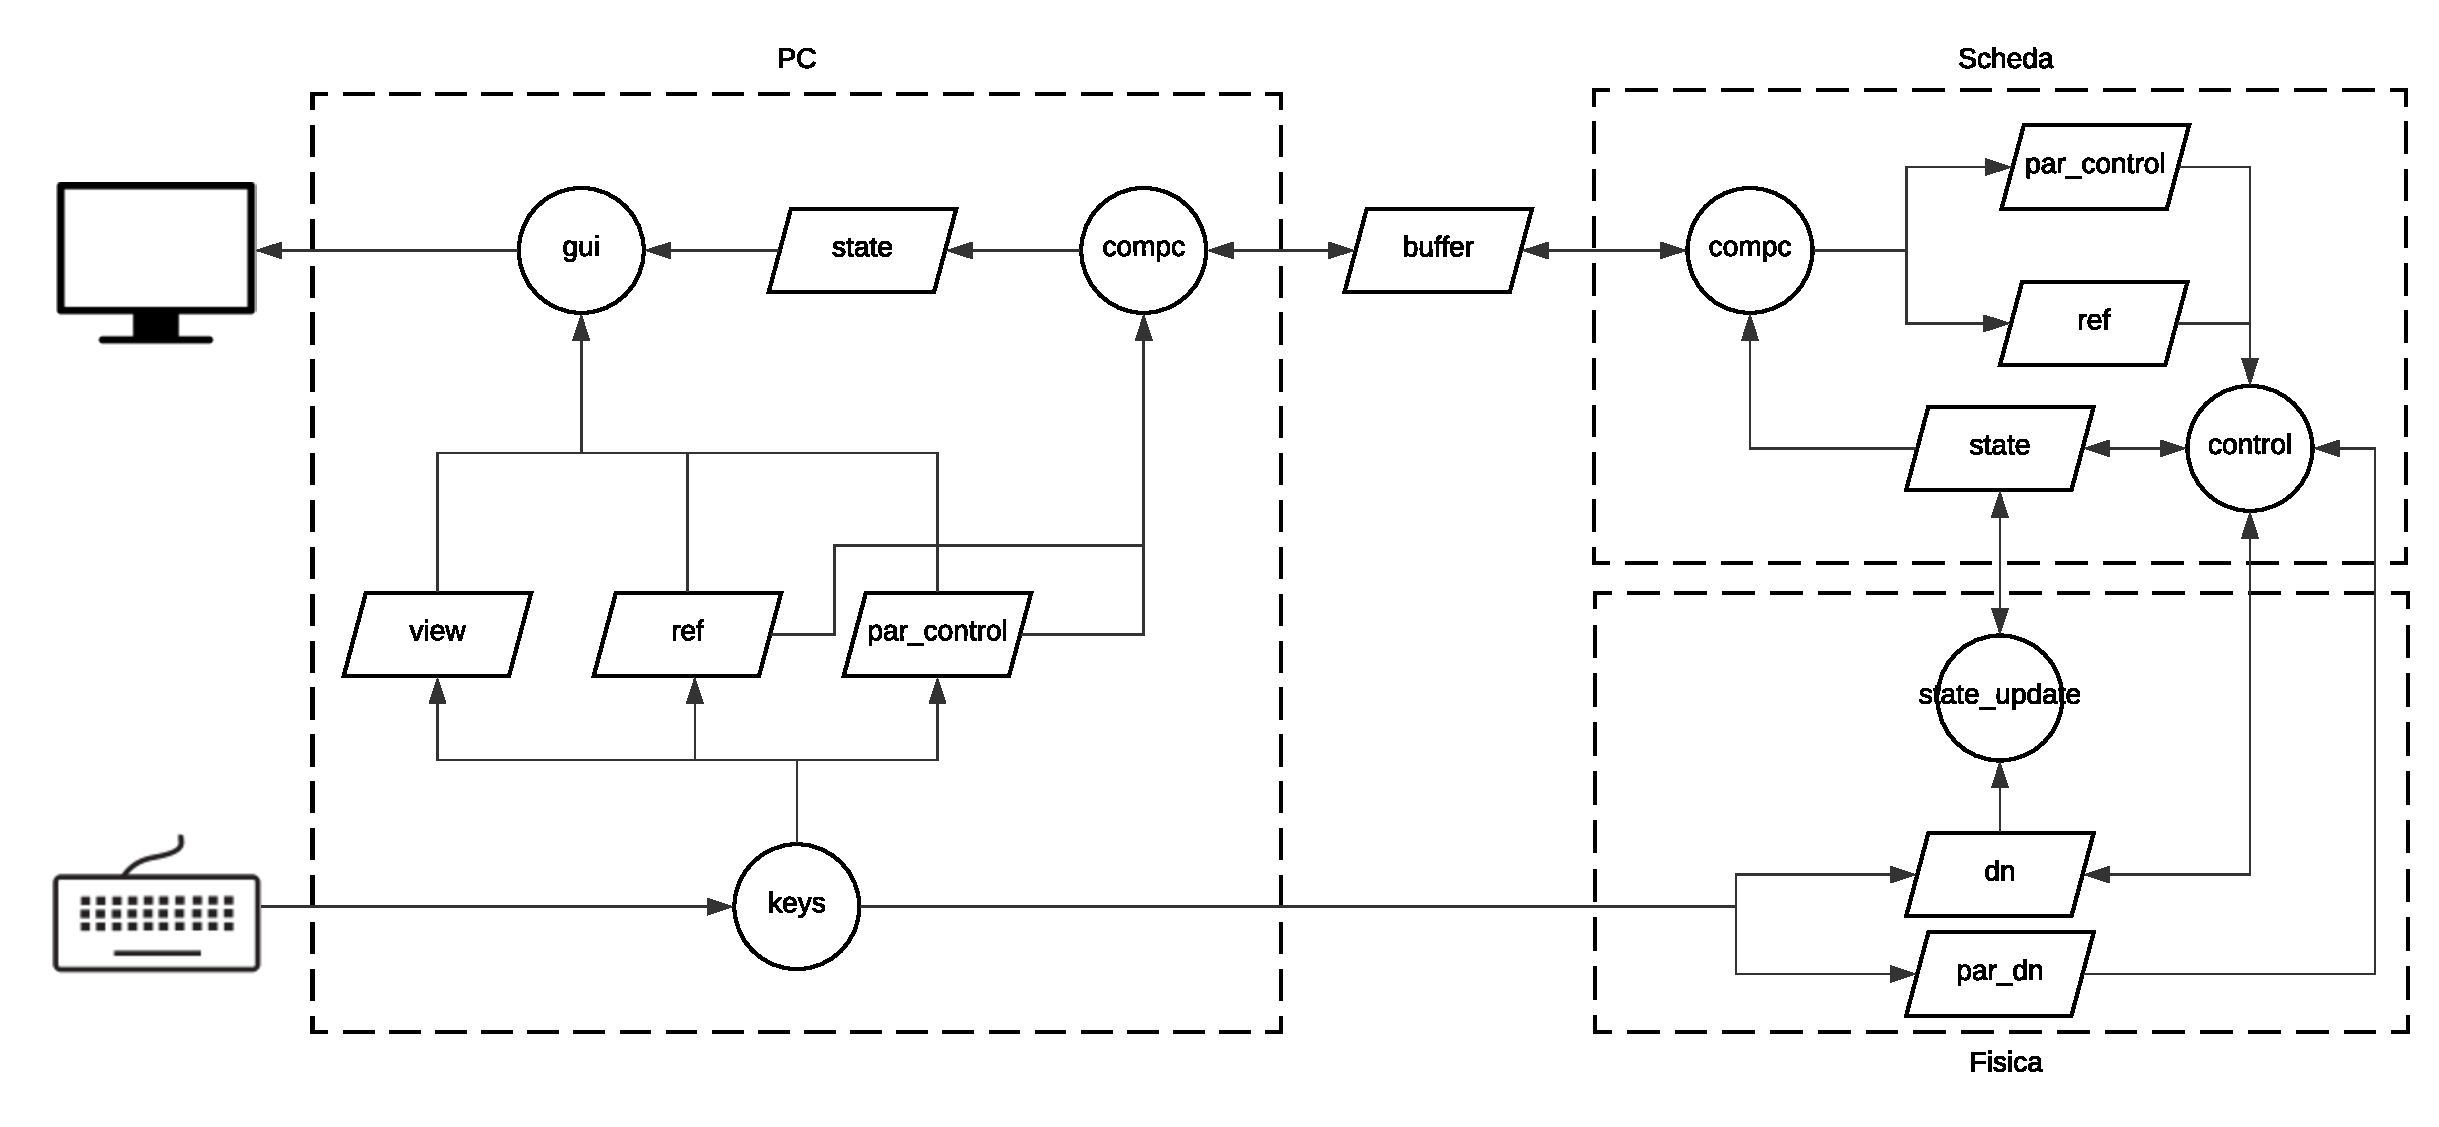
\includegraphics[width=\linewidth]{diagramma_task_risorse.pdf}
	\caption{Diagramma delle risorse e dei task}
	\label{fig:risorse_task}
\end{figure}

L'idea base nella suddivisione dei task \`e stata il voler separare l'interfaccia pc dalla simulazione della scheda e dalla simulazione della fisica del pendolo. A tal proposito sono stati creati i seguenti task:
\begin{itemize}
	\item \textit{state\_update}, aggiorna lo stato in base al modello descritto nella sezione~\ref{sez:modello}
	\item \textit{control}, legge lo stato e il riferimento e modifica l'azione di controllo in base alle leggi sviluppate nella sezione~\ref{sez:controllo}
	\item \textit{comboard}, comunica tra scheda e il buffer condiviso
	\item \textit{compc}, comunica tra pc e il buffer condiviso
	\item \textit{keys}, legge che tasti vengono premuti e compie azioni di conseguenza
	\item \textit{gui}, disegna e aggiorna l'interfaccia utente esposta nella sezione~\ref{sez:interfaccia}
\end{itemize}

\begin{table}[h]
	\centering
	\begin{tabular}{rcc}
		\multicolumn{1}{c}{Task}                & Periodo      & Priorit\`a \\ \hline
		\textit{state\_update} & $\SI{1}{\ms} $  & 99         \\
		\textit{control}      & $\SI{5}{\ms} $ & 90         \\
		\textit{comboard}     & $\SI{5}{\ms} $ & 30         \\
		\textit{compc}        & $\SI{5}{\ms} $ & 30         \\
		\textit{keys}         & $\SI{20}{\ms}$ & 20         \\
		\textit{gui}          & $\SI{40}{\ms}$ & 10         \\ 
	\end{tabular}
\caption{Priopriet\`a task}
\label{tab:info_task}
\end{table}

Per differenziare ulteriormente le simulazioni delle varie componenti \`e stata assegnato un diverso core della CPU ad ogni componente. Si ha quindi \textit{state\_update} su un processore a lui dedicato, \textit{control} e \textit{comboard} su un secondo e infine \textit{keys}, \textit{compc} e \textit{gui} su un terzo.

\subsubsection{\textit{state\_update}}
Questo task si occupa di simulare la fisica del pendolo. Essendo impossibile eseguire l'aggiornamento dello stato in modo continuo, la velocit\`a di esecuzione \`e molto importante per approssimare in modo appropriato il modello discreto a quello continuo. Per questo motivo \`e il task di maggior priorit\`a e con minore tempo di esecuzione.

La funzione principale di questo task \`e \texttt{physics} ottenuta tramite il generatore di codice di \textsc{Simulink--Matlab}.
\textit{Altro?}

\subsubsection{\textit{control}}
I suoi scopi sono quelli di simulare le azioni del microcontrollore tramite la funzione \texttt{controller} e quello di aggiornare la structure \texttt{dn} per mezzo della funzione \texttt{disturbance and noise}. 

Le funzioni \texttt{controller} e \texttt{disturbance and noise} sono state ottenute dall'uso dell'em\-bed\-ded coder di \textsc{Simulink--Matlab}. La prima, con alcune modifiche, \`e la funzione da caricare sul microcontrollore stesso. La priorit\`a di \textit{control} \`e secondaria solo alla simulazione fisica.
 
\textit{SCRITTO A CULO, Altro?}

\subsubsection{\textit{compc} e \textit{comboard}}
Questi sono i due task di comunicazione, \textit{compc} lato pc e \textit{comboard} lato scheda. Il primo si occupa di scrivere il riferimento e i vari parametri di controllo sul buffer e di leggere lo stato del pendolo in memoria sul buffer. Il secondo in modo opposto, legge il riferimento e i parametri di controllo e scrive lo stato.

\subsubsection{\textit{keys}}
Si occupa delle varie interazioni tra tastiera e le strutture dati a cui si ha accesso lato pc. I vari tasti che modificano riferimento, parametri e vista sono visibili nell'interfaccia sia accanto alla variabile che vanno a modificare sia in basso per i tasti di reset.

\textit{Altro?}

\subsubsection{\textit{gui}}
Scrive su schermo tutte le statistiche relative ai task, i parametri, i riferimenti e lo stato. Inoltre si occupa di disegnare le varie viste descritte nella sezione~\ref{sez:interfaccia}. 

A differenza dei precedenti questo task non \`e coinvolto nella simulazione del pendolo, la sua esecuzione \`e quindi secondaria e il suo periodo pu\`o essere rilassato fino a valori che siano sufficienti a visualizzare le informazioni su schermo senza troppa latenza. Il periodo \`e stato quindi scelto per avere 25 frame al secondo.














\FloatBarrier

\section{Conclusioni (?)}
Da Scrivere?

	
\end{document}